% =========================================================================
%  P1 -- Reproducible benchmark, clock calibration, cross-port audit
%  IEEEtran journal manuscript.  Result tables are \input.
% =========================================================================
\documentclass[journal,10pt]{IEEEtran}

\usepackage[utf8]{inputenc}
\usepackage[T1]{fontenc}
\usepackage{amsmath,amssymb,amsthm}
\usepackage{graphicx}
\usepackage{booktabs}
\usepackage{multirow}
\usepackage{array}
\usepackage{subcaption}
\usepackage{algorithm}
\usepackage{algpseudocode}
\usepackage{url}
\usepackage{cite}
\usepackage{xcolor}
\usepackage{balance}

\graphicspath{{../results/figures/}{diagrams/}}

\newtheorem{proposition}{Proposition}
\newcommand{\bigO}{\ensuremath{\mathcal{O}}}

\hyphenation{Pure-Edge-Sim re-pro-duc-i-bil-i-ty bench-mark bench-marks}

\begin{document}

\title{Temporal Resolution and Architectural Effects in Edge Computing
Simulations: A Common-Scenario Cross-Simulator Benchmark and Calibration Framework}

\author{Anonymous Authors%
\thanks{Manuscript prepared for review. Every table is generated from the
released artifact; the clock experiment of Section~\ref{sec:clock} is
reproducible from the shipped settings.}}

\markboth{IEEE Transactions on Mobile Computing (submitted)}%
{What the Clock Does to Edge Simulation}

\maketitle

\begin{abstract}
A crossed benchmark of $3{,}215$ seeded executions reports what looks like a
clean architectural result: edge-only placement succeeds on $0.121$ of requests
and a full mist/edge/cloud deployment on $0.660$, a difference eight times
larger than quadrupling the fleet. This paper shows that this number is an
artefact of the simulator's control interval. Class decomposition first shows
that the edge-only ratio equals the share of requests whose deadline exceeds one
second: infrastructure placements wait $1.01$--$2.12$~s before execution because
the orchestrator runs on a $1$~s tick, so every $0.2$~s and $0.8$~s task fails
there, while the $60$~s class survives. Adding the mist tier helps only because
peer devices start work at release. A controlled sweep of the interval confirms
the mechanism: at $1$~s the architecture effect is $0.539$, at $0.2$~s it is
$0.415$, and at $50$~ms it is $-0.004$. Scaling every deadline by $16$ returns
the effect to $0.011$, and varying the class mix moves edge-only success to the
aggregation share exactly ($0.030$, $0.068$, $0.121$, $0.186$, $0.444$). The
scheduling lag tracks the interval ($1.01$, $0.21$, $0.06$~s), so the causal
chain is measured rather than inferred.

The artefact had hidden the real question, which is when the architectural
choice is genuine. Crossing four infrastructure profiles with seven
orchestration algorithms and two control intervals ($1{,}680$ runs) answers it:
at $1$~s the effect is $+28$ to $+34$ points under \emph{every} profile,
including one where the cloud is slow and distant, whereas at $50$~ms its sign is
predicted by the profile: $+65.7$ points when the edge is weak and the cloud
fast, $-3.6$ to $-19.6$ when the edge is already adequate. The same design shows
that algorithm rankings are not configuration-free: the weakest cross-interval
rank agreement is Kendall $\tau=0.103$, the winner changes with the
infrastructure, and least-loaded placement moves from first to last. We replace
the ``interval $\le D/10$'' rule of thumb with a measured calibration: success is
stable while the decision latency stays below half the deadline and collapses
once it exceeds it. Deciding costs $0.15$--$0.52$~ms per task, $0.6$--$3.0\%$ of
runtime, so the wait is the clock and not the algorithm. Four trace arms and an
independent simulator replication bound how far the synthetic conclusions
travel. A common application graph, a shared trace and a source-verified
capability matrix make the cross-platform comparison explicit rather than
assumed: on that common scenario YAFS reproduces the artefact ($+47.6$ points at
$1$~s, zero at $50$~ms), whereas EdgeCloudSim has no global periodic loop and
serves every class, so the phenomenon is conditional on an engine's temporal
semantics rather than universal. Energy per success is shown to be denominator-driven, and a Java/Python
audit at version parity localises the residual divergence to wide-area
accounting.
\end{abstract}

\begin{IEEEkeywords}
Benchmarking, simulation calibration, control interval, edge orchestration,
reproducibility, workload feasibility, simulator portability.
\end{IEEEkeywords}

% =========================================================================
\section{Introduction}
\label{sec:intro}

A reader of the 2026 edge-computing literature is asked to compare mechanisms
evaluated under incomparable conditions: different topologies, different link
rates, different workload generators, and different simulator
configurations. Nothing in a typical results section lets the reader decide
whether a reported difference is the mechanism, the architecture, the workload,
or the simulator's configuration.

The obvious remedy is a crossed benchmark: hold the simulator fixed, vary the
factors papers argue about, and let effect sizes speak. This paper reports such
a benchmark, the conclusion it produced, and the experiment that overturned it.

\subsection{Research questions}
We separate three objectives that a single-simulator study cannot distinguish:
\emph{calibration} (does temporal resolution distort outcomes?),
\emph{cross-simulator validation} (does the effect survive a different engine?),
and \emph{application and infrastructure validation} (does it survive
dependencies, realistic workloads and heterogeneous capacity?). They map to:

\begin{description}
\item[RQ1.] How does temporal resolution influence performance measurements in
  edge-computing simulation scenarios?
\item[RQ2.] To what extent do the observed effects depend on the temporal and
  scheduling semantics of different edge-computing simulators?
\item[RQ3.] How do application characteristics, workload composition, resource
  heterogeneity and network conditions affect simulation outcomes?
\item[RQ4.] How stable are the rankings of orchestration and placement algorithms
  across simulation configurations and infrastructure scenarios?
\item[RQ5.] What calibration and reproducibility procedures are necessary to make
  results comparable across edge-computing simulators?
\end{description}

RQ1 and RQ4 are answered by the crossed PureEdgeSim grids; RQ2 by the
common-scenario adapters of Section~\ref{sec:common}; RQ3 by the dependency-aware
application model and the heterogeneity/trace grids; RQ5 by the measured
latency-to-deadline ratio of Section~\ref{sec:calibration}. The Java/Python
port audit is reported separately from cross-simulator evidence: the two ports
are one framework, not two simulators.

The scope is **edge-computing simulation**, not multi-tier orchestration as a
research domain. The mist/edge/cloud infrastructure studied here is one
deployment scenario; Section~\ref{sec:app-model} defines its application graph
and Section~\ref{sec:infra-model} its topology. Nothing in the paper assumes that
edge-computing scenarios in general contain all three classes of resource, and
the deployment configurations of Section~\ref{sec:infra-model} are experimental
factors rather than a taxonomy of the field.

\subsection{The result, and what it was measuring}
The benchmark crosses five factor families over $3{,}215$ seeded runs. Read at face
value, it says that \emph{architecture dominates scale}. At $40$ devices with
the simulator's default trade-off policy, edge-only placement succeeds on
$0.121$ of requests and a full mist/edge/cloud deployment on $0.660$; a
four-fold increase in fleet size moves success by at most $0.065$. The
architecture effect is $0.539$, between eight and fifteen times the scale
effect.

Decomposing by class shows that edge-only succeeds on exactly one class: the
$60$~s aggregation jobs, which are $0.121$ of the request mix and succeed on
$0.975$ of attempts. The $0.2$~s sensing and $0.8$~s video classes succeed on
$0.000$ under both lower architectures. Recomposing,
$0.121\times0.975+0.528\times0.779+0.352\times0.374=0.661$, which matches the
pooled $0.660$. The ``architecture gain'' is the share of the workload that can
use the mist tier.

The natural reading is a feasibility boundary: hard classes fit on mist peers
but not on infrastructure. That reading is wrong, and the delay records say so.
Under the full architecture, a sensing task placed on an edge data centre runs
in $0.025$~s, well inside its $0.2$~s deadline, and still fails. What it cannot
absorb is the wait: execution starts $1.01$~s after release on an edge site and
$2.12$~s after release in the cloud, because the orchestrator is invoked on a
one-second tick. The $60$~s class tolerates that wait; the other two do not.

The control interval, not the architecture, sets the result. We test this
directly by sweeping the interval with everything else fixed. At $1$~s the
effect is $0.539$; at $0.2$~s it is $0.415$; at $50$~ms it is $-0.004$, with
edge-only at $0.987$ and the full architecture at $0.983$. The scheduling lag
tracks the interval ($1.01$, $0.21$, $0.06$~s), and success tracks the lag.
The effect is a simulation artefact, and it is monotone in the parameter that
causes it.

\subsection{Why this is worth reporting}
The failure mode is silent. The simulator runs, the tables are produced, the
differences are large and statistically clean, and the conclusion is plausible
enough to publish. Nothing in the output says ``the clock is the treatment''.
Our own first draft reported the effect as a finding; the correction came from
asking why a task that finishes in $0.025$~s misses a $0.2$~s deadline.

The lesson generalises beyond this simulator. Any discrete-event evaluation of
sub-second services has a control interval, and that interval must be an order
of magnitude below the tightest deadline before placement or policy differences
can be attributed to the mechanism under test. We state this as a calibration
rule with a checklist
(Section~\ref{sec:calibration}), and we show what survives once it is applied.

\subsection{Contributions}
\begin{enumerate}
\item A simulator-independent benchmark specification---application DAG,
  workload trace, topology, deployment eligibility, reference policies and
  common metrics---together with adapters that consume the same trace, and a
  source-verified capability matrix for the four platforms discussed
  (Sections~\ref{sec:design}, \ref{sec:common}; \texttt{crosssim/SPEC.md},
  \texttt{CAPABILITIES.md}).
\item A common-scenario temporal calibration on two independent engines: YAFS
  reproduces the artefact ($+47.6$ points at $1$~s, zero at $50$~ms), while
  EdgeCloudSim, which has no global periodic loop, serves every class and cannot
  exhibit it---turning the claim from a single-simulator observation into a
  conditional cross-simulator result (Section~\ref{sec:common}).
\item A $3{,}215$-run crossed benchmark with fixed statistics and an artifact
  from which every table is generated (Sections~\ref{sec:design},
  \ref{sec:method}).
\item A class decomposition that reduces the pooled architecture effect to the
  share of requests with deadlines below the control interval
  (Section~\ref{sec:decompose}).
\item A controlled interval sweep, a deadline-scaled sweep and a class-mix
  sweep that turn the explanation into a measured causal chain and show the
  effect vanishing at $50$~ms (Sections~\ref{sec:clock}--\ref{sec:mix}).
\item A crossed algorithm $\times$ architecture $\times$ interval design
  ($630$ runs) showing that algorithm rankings do not survive a change of
  temporal configuration, quantified with Kendall $\tau$ and a factorial ANOVA
  (Section~\ref{sec:algos}).
\item An infrastructure-heterogeneity experiment ($1{,}680$ runs) that
  separates the artefact from the phenomenon: the architecture effect changes
  sign with the clock and is predicted by the capacity gap between tiers
  (Section~\ref{sec:hetero}).
\item A calibration procedure in which the ``$D/10$'' rule is replaced by a
  measured relation between orchestration decision latency and deadline, with
  the latency decomposed into release, decision, dispatch and execution
  (Section~\ref{sec:calibration}).
\item A four-arm workload-realism study and an independent-simulator
  replication that bound the external validity of the synthetic conclusions
  (Sections~\ref{sec:trace}--\ref{sec:crosssim}).
\item Four results that survive the correction: the energy denominator effect,
  the conditional mobility effect, the measured cost of deciding, and a
  three-level cross-port audit that localises a real divergence to WAN
  accounting (Sections~\ref{sec:energy}--\ref{sec:parity}).
\end{enumerate}

% =========================================================================
\section{Related Work}
\label{sec:related}

\subsection{Edge orchestration}
The architectural question---which tiers should participate---is as old as edge
computing~\cite{satyanarayanan2017,shi2016edge}, and MEC
surveys~\cite{mao2017survey,mach2017survey} already note that the answer depends
on the workload mix. Game-theoretic offloading~\cite{chen2015game} and
Pareto-aware reinforcement learning~\cite{xu2026paretoRL} optimise the choice of
tier; our benchmark asks how much the \emph{available set} matters before any
optimiser is applied, and finds that in a mis-calibrated simulator it matters
for a reason unrelated to optimisation.

\subsection{Benchmarking methodology}
The pitfalls of systems benchmarking are well documented: Hoefler and Belli
catalogue twelve ways in which performance comparisons mislead, including
inappropriate simulators and hidden configuration
effects~\cite{hoefler2015benchmarking}, and benchmark suites such as
TailBench~\cite{kasture2016tailbench} and MLPerf~\cite{reddi2020mlperf} exist
precisely because a poorly chosen workload can dominate the measured difference.
When seeds are reused across arms, common random numbers reduce variance but
also change the correct analysis~\cite{glasserman1992common}, which is why we
report seed-matched tests alongside the pooled ones. Simulation model verification and
validation has its own literature, which insists that a model be shown to
represent the system before its outputs are interpreted~\cite{sargent2013verification}.
Our contribution is an instance of both: a configuration parameter that is
usually left at its default silently defines the treatment, and the model's
output is interpretable only after the parameter is calibrated against the
deadlines it is supposed to resolve.

\subsection{Simulator ecosystem}
CloudSim~\cite{calheiros2011cloudsim} established the discrete-event pattern;
PureEdgeSim~\cite{mechalikh2021pureedgesim} extends it with mist nodes, mobility
and per-link energy. The wider ecosystem---iFogSim~\cite{gupta2017ifogsim} and its mobility/microservice
extension~\cite{mahmud2022ifogsim2},
EdgeCloudSim~\cite{sonmez2018edgecloudsim},
YAFS~\cite{lera2019yafs}---shares the same discrete-event structure and
therefore the same class of calibration hazard: each has an update or scheduling
interval whose default is chosen for second-scale workloads. Our result should
be read as a warning for all of them, not only for the one we ran.

\subsection{Trace-driven evaluation}
Trace replay has a long tradition in caching and
storage~\cite{breslau1999caching}, and the LLM serving
literature now provides production traces and phase-level
models~\cite{patel2024splitwise,shahrad2020serverless}. Replaying such a trace
is only meaningful if the mapping from trace units to simulated work is stated;
we give ours explicitly and treat the result as a calibration check rather than
as a workload claim.

% =========================================================================
\section{Benchmark Design}
\label{sec:design}

This section follows the reviewer's separation of simulator platforms,
application/workload, and infrastructure/deployment. Figures~\ref{fig:app},
\ref{fig:topo} and \ref{fig:deploy} establish the model independently of any
simulator; the machine-readable sources are
\texttt{crosssim/application\_graph.json}, \texttt{crosssim/scenario.json} and
\texttt{crosssim/traces/}.

\subsection{Application and dependency model}
\label{sec:app-model}
We use a UAV-assisted surveillance scenario with five services. Data acquisition
(S1) produces a class-dependent sample; preprocessing (S2) and feature extraction
(S3) transform it; event detection (S4) makes the hard-deadline decision; and
aggregation (S5) rolls results up. Three workflows compose these services:
C1 = S1$\to$S2$\to$S4 (0.20~s, 2{,}000~MI),
C2 = S1$\to$S2$\to$S3$\to$S4$\to$S5 (0.80~s, 12{,}000~MI), and
C3 = S1$\to$S5 (60~s, 20{,}000~MI). Each DAG edge carries its parent's output as
the child's input and pays the inter-tier link cost when the two services are
placed on different nodes.

\begin{figure}[t]
\centering
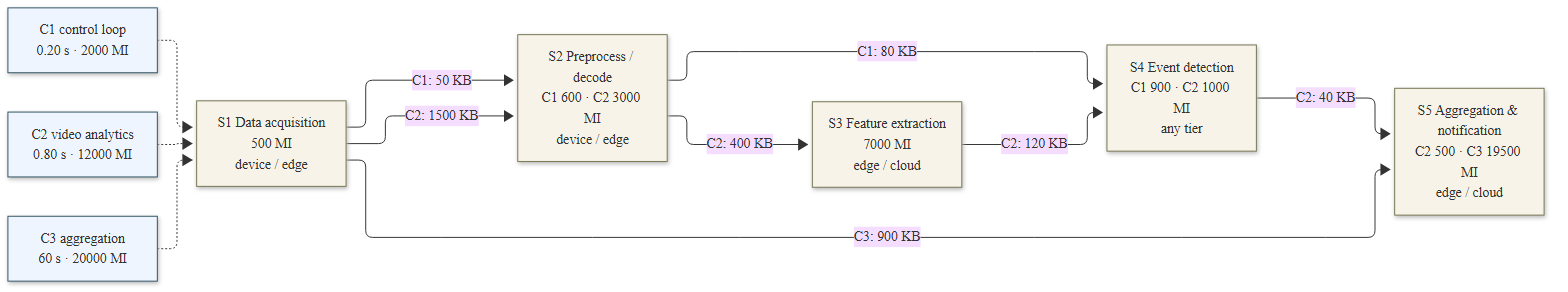
\includegraphics[width=\columnwidth]{application_graph.png}
\caption{Application graph. Services are independent of the infrastructure;
edges are data dependencies with the sizes used by the adapters.}
\label{fig:app}
\end{figure}

This model answers the reviewer's dependency question directly. The original
three-class workload is the \emph{independent} arm, in which each workflow's
services are collapsed into one task; the \emph{workflow} arm releases each
service separately and measures workflow completion, dependency violations and
intermediate transfer cost. The common trace generator asserts that each
workflow's service MI sums to its class total.

\subsection{Infrastructure and deployment configurations}
\label{sec:infra-model}
The topology is fixed: 40 devices (16 UAV at 30{,}000~MIPS, 16 field units at
12{,}000~MIPS, 8 sensors with no compute), three edge data centres of 16 cores
at 80{,}000~MIPS, and one cloud of 400 cores at 100{,}000~MIPS. Wi-Fi links are
300~Mb/s/10~ms, the MAN 1{,}000~Mb/s/10~ms and the WAN 50~Mb/s/120~ms. The
global orchestrator sits at an edge node and is triggered at the control
interval.

\begin{figure}[t]
\centering
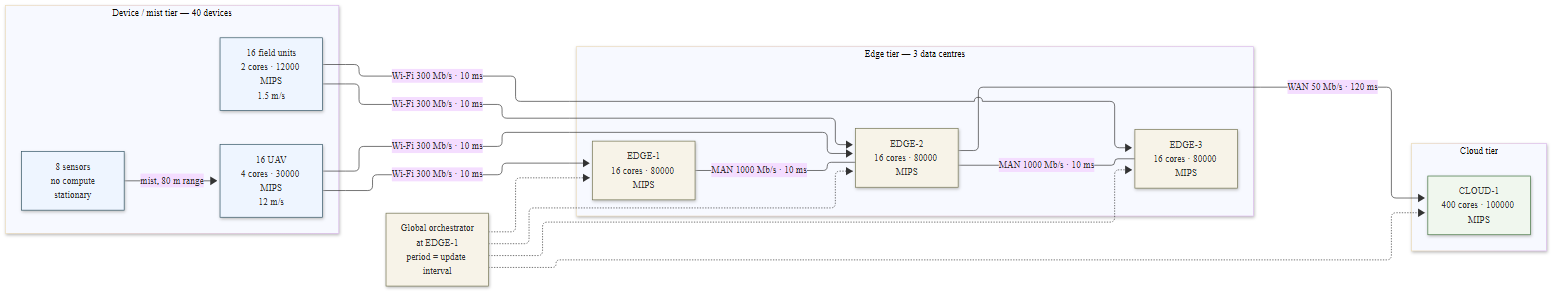
\includegraphics[width=\columnwidth]{infrastructure.png}
\caption{Infrastructure topology. Tier capacities, link rates and the
orchestrator's location are fixed across the deployment arms.}
\label{fig:topo}
\end{figure}

\begin{figure}[t]
\centering
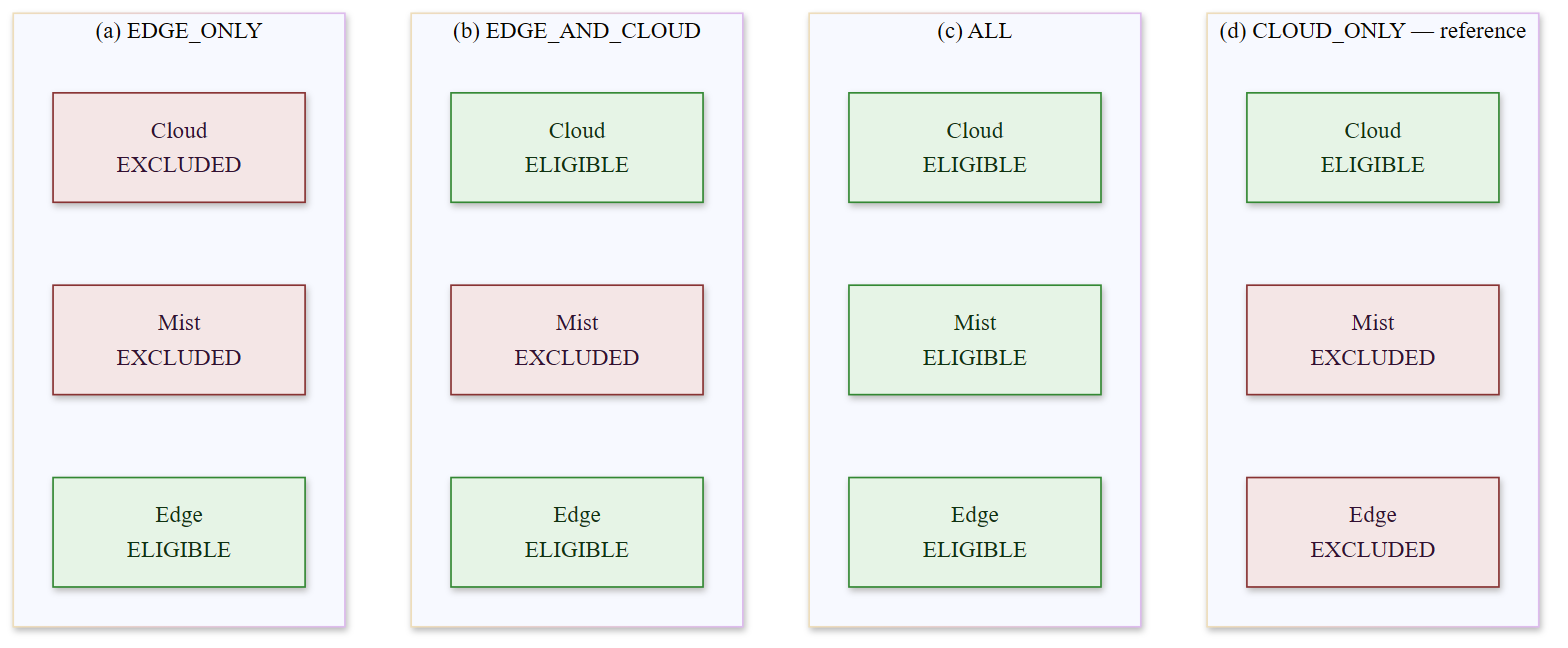
\includegraphics[width=\columnwidth]{deployments.png}
\caption{Deployment configurations. Eligibility changes; the physical nodes do
not. EDGE\_AND\_CLOUD differs from ALL only in mist eligibility.}
\label{fig:deploy}
\end{figure}

\subsection{Simulator platforms and temporal semantics}
Five platform instances are discussed: PureEdgeSim Python and Java (one
framework, two ports), YAFS 3.1, EdgeCloudSim and iFogSim2. Only the first two
are the same simulator. PureEdgeSim exposes a periodic global tick
(\texttt{update\_interval}); YAFS has native event-driven routing and our adapter
injects the equivalent tick; EdgeCloudSim and iFogSim2 place at task/deployment
time and offer no global period. These are documented capability facts
(\texttt{crosssim/CAPABILITIES.md}), not hidden differences. The benchmark
pipeline in Figure~\ref{fig:pipeline} shows where the global control loop sits
and which stages the calibration procedure measures.

\begin{figure*}[t]
\centering
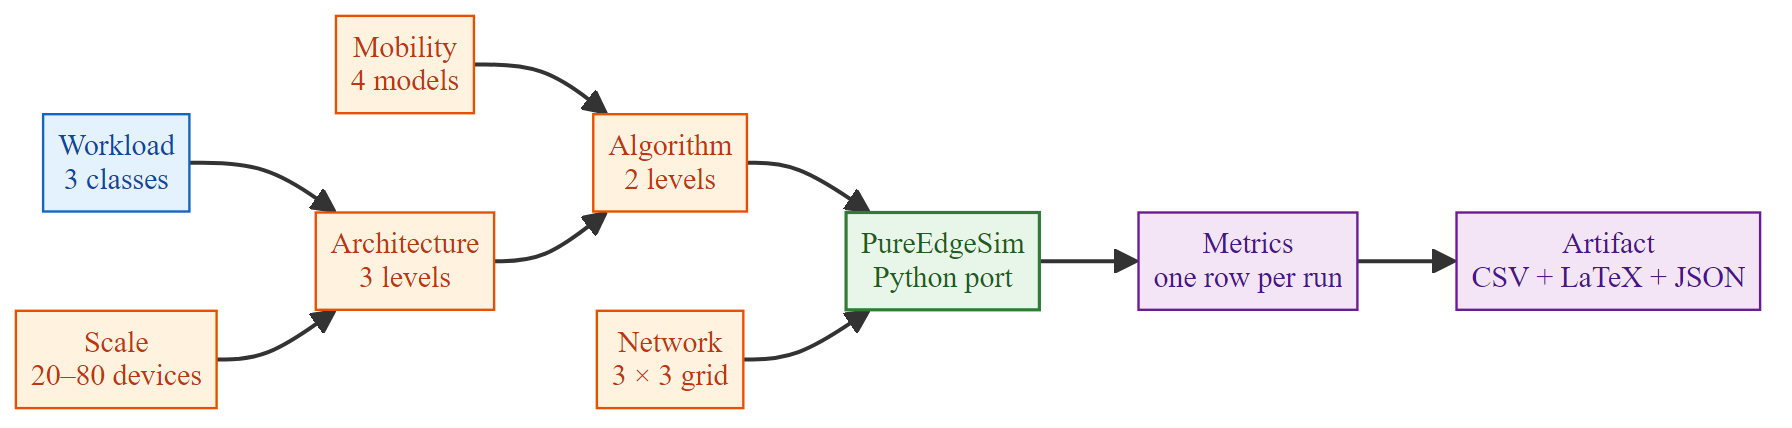
\includegraphics[width=0.92\textwidth]{pipeline.png}
\caption{Benchmark pipeline. Factor families (orange) are crossed; the
simulator and the metric definitions are held fixed; every run emits one row
and every table in this paper is generated from those rows.}
\label{fig:pipeline}
\end{figure*}

\subsection{Simulator and infrastructure}
The benchmark runs on the Python port of PureEdgeSim 6.1.0 (the port maintained
with the simulator, not a third-party rewrite), an event-driven simulator of
cloud/edge/mist hierarchies. Table~\ref{tab:p1-infra} lists the infrastructure.
Three edge data centres provide $80{,}000$~MIPS across $16$ cores each and the
cloud provides $100{,}000$~MIPS across $400$ cores; the task records show that a
task is charged the node's aggregate throughput rather than a single core, which
is why we report measured lags and delays instead of a per-core bound.

\begin{table}[t]
\centering
\footnotesize
\caption{Infrastructure and links (from \texttt{settings/*.xml}). Device
percentages are of the fleet; sensors have no compute and must offload.}
\label{tab:p1-infra}
\begin{tabular}{@{}lccc@{}}
\toprule
Tier & Count & Cores & MIPS\\
\midrule
Edge device, class A & 40\% & 4 & 30{,}000\\
Edge device, class B & 40\% & 2 & 12{,}000\\
Sensor (no compute) & 20\% & 0 & 0\\
Edge data centre & 3 & 16 & 80{,}000\\
Cloud data centre & 1 & 400 & 100{,}000\\
\midrule
\multicolumn{4}{@{}l}{WiFi 300 Mb/s, 10 ms; WAN 50 Mb/s, 120 ms; MAN 1 Gb/s}\\
\multicolumn{4}{@{}l}{Realistic network model on; placement cache at default}\\
\bottomrule
\end{tabular}
\end{table}

Three configuration choices are part of the protocol because they change
results and are usually left implicit: the realistic network model is enabled;
the per-device placement cache is left at its default, which is what a
reproducer would obtain; and the control interval is the object of study in
Section~\ref{sec:clock} rather than a hidden constant.

\subsection{Workload}
Three classes proxy a multi-tier deployment (Table~\ref{tab:p1-workload}). They
span three orders of magnitude in deadline, which is what makes the workload
sensitive to the control interval: two of the three deadlines are shorter than
the simulator's default tick.

\begin{table}[t]
\centering
\footnotesize
\caption{Workload classes (per generating device), from
\texttt{applications.xml}. ``Share'' is the resulting fraction of generated
requests.}
\label{tab:p1-workload}
\begin{tabular}{@{}lccc@{}}
\toprule
 & Sensing & Video & Aggregation\\
\midrule
Class & hard RT & soft RT & non RT\\
Rate (req/min) & 15 & 10 & 4\\
Deadline (s) & 0.20 & 0.80 & 60.0\\
Length (MI) & 2{,}000 & 12{,}000 & 20{,}000\\
Container (kB) & 200 & 1{,}200 & 800\\
Result (kB) & 20 & 60 & 100\\
Device share & 35\% & 35\% & 30\%\\
Share of requests & 0.528 & 0.352 & 0.121\\
\bottomrule
\end{tabular}
\end{table}

\subsection{Factors}
\emph{Architecture} $\in$ \{\textsc{edge\_only}, \textsc{edge\_and\_cloud},
\textsc{all}\}: the set of tiers eligible to host a task.
\emph{Algorithm} $\in$ \{\textsc{trade\_off}, \textsc{round\_robin}\}.
\emph{Scale} $\in$ $\{20,40,60,80\}$ devices from the same fleet definition.
\emph{Mobility} $\in$ \{random-waypoint, Gauss--Markov, waypoint, group\}.
\emph{Network} $\in$ WAN latency $\{0.03,0.12,0.30\}$~s $\times$ WiFi bandwidth
$\{50,300,1300\}$~Mbps.
\emph{Control interval} $\in$ $\{1.0, 0.2, 0.05\}$~s, added after the main grid
and analysed in Section~\ref{sec:clock}.

\subsection{Generators}
The synthetic generator draws inter-arrival times from
Table~\ref{tab:p1-workload}. The trace generator replays a public Azure LLM code
trace, taking every record with arrival below the $300$~s horizon ($781$
requests) and mapping it linearly to a task:
\begin{equation}
\begin{aligned}
w &= 500+2c+8g &&\text{(MI)},\\
b_{\text{req}} &= 0.5+0.002c &&\text{(kB)},\\
b_{\text{res}} &= 0.1+0.004g &&\text{(kB)},
\end{aligned}
\label{eq:trace}
\end{equation}
with deadline $\max(0.5,\,2+5\times10^{-4}c)$ seconds, where $c$ and $g$ are the
context and generated token counts. Classes are assigned round-robin, so the
trace arm is class-balanced rather than mix-preserving; this is a limitation of
the comparison, not a property of the trace.

\subsection{Determinism}
Every run is seeded. A determinism check re-ran one configuration and compared
four aggregates; the values were identical. Across architectures the device list
is unchanged, so the generator's random stream is identical; across fleet sizes
it is not, which is a caveat on cross-scale comparisons.

% =========================================================================
\section{Methodology}
\label{sec:method}

\subsection{Grids}
Table~\ref{tab:p1-grids} lists the grids: $3{,}215$ runs of five simulated
minutes, ten seeds per cell (five for the network grid).

\begin{table}[t]
\centering
\small
\caption{Benchmark grids and run counts.}
\label{tab:p1-grids}
\begin{tabular}{@{}lccc@{}}
\toprule
Grid & Factors & Cells & Runs\\
\midrule
scale & arch $\times$ alg $\times$ devices & $3\times2\times4$ & 240\\
mobility & model $\times$ arch & $4\times3$ & 120\\
trace & workload $\times$ arch & $4\times3$ & 120\\
network & WAN $\times$ WiFi $\times$ arch & $3\times3\times3$ & 135\\
clock & arch $\times$ interval & $3\times3$ & 90\\
deadline & arch $\times$ deadline mult. & $2\times5$ & 100\\
mix & arch $\times$ class mix & $2\times5$ & 100\\
algo & alg $\times$ arch $\times$ interval & $7\times4\times3$ & 630\\
hetero & profile $\times$ alg $\times$ interval & $4\times7\times6$ & 1680\\
\midrule
\multicolumn{3}{@{}l}{Total} & 3215\\
\bottomrule
\end{tabular}
\end{table}

The \texttt{algo} grid crosses seven orchestration algorithms with four
architecture levels and three control intervals. The four architecture levels
are the three substantive configurations plus a pooled \textsc{all} level that
is the same runs read without the mist/edge/cloud split, so the design is
balanced at $7\times3\times3\times10$ substantive runs. The \texttt{hetero} grid
crosses four capacity profiles with the same seven algorithms, three
architectures and two intervals. Both are analysed with a factorial model rather
than one contrast at a time, because the review question is precisely whether
the effects interact.

\subsection{Metrics}
\emph{Success ratio} is successful tasks divided by generated tasks; a task
succeeds only if it executes and its result returns before its own latency
bound. \emph{p95 delay} is the $95$th percentile of delivery delay over
\emph{successful} tasks, which makes it a survivorship statistic: a policy that
refuses hard tasks will appear to have a short tail, and we therefore read p95
only alongside success and the per-class budget of
Table~\ref{tab:p1-budget}. \emph{Energy per success} divides computing-node
energy by successful tasks; network energy is reported separately by the
simulator and excluded, and we state that boundary because including it would
change the comparison. \emph{Energy per generated task} divides the same
numerator by generated tasks and exists because the first metric is
denominator-driven. \emph{WAN usage} is cumulative wide-area link occupancy.
\emph{Runtime} is harness wall-clock time.

\subsection{Statistics}
Each arm has ten seeded runs. We report means with bootstrap $95\%$ confidence
intervals of the difference, Mann--Whitney $U$ tests with Holm--Bonferroni
correction, and Cliff's $\delta$. Two caveats are stated rather than buried.
First, Mann--Whitney assumes independent samples; the seeds are reused across
arms but the test treats arms as independent, which is conservative when the
pairing is positive. Second, when a control arm has zero variance---as
\textsc{edge\_only} does for success at a fixed interval---Cliff's $\delta$ is
trivially $\pm1$ and the bootstrap interval reflects treatment variance only; we
print the value but do not interpret it.

\subsection{Artifact}
The artifact contains the settings, job dictionaries, one CSV per run, the
per-task records, aggregate tables, the \LaTeX{} tables used here, figures, a
data dictionary and a manifest. This manuscript \verb|\input|s the shipped
tables.

% =========================================================================
\section{Results}
\label{sec:results}
% Anchors retained for cross-references from the model, methodology and discussion.
\label{sec:decompose}\label{sec:clock}\label{sec:deadline}\label{sec:mix}
\label{sec:algos}\label{sec:hetero}\label{sec:energy}\label{sec:trace}
\label{sec:parity}\label{sec:crosssim}\label{sec:common}\label{sec:calibration}

This section is organised around the research questions. Every value quoted is
recomputed from the run tables; the exact subset and averaging method are stated
where several closely related effects exist. Detailed numerical matrices and
full statistical output are in the supplementary file.

\subsection{Baseline performance and fleet-size sensitivity}
Figure~\ref{fig:new-f4} reports the main performance results. At $40$ devices
with \textsc{trade\_off}, \textsc{edge\_only} and \textsc{edge\_and\_cloud} both
succeed on $0.121$ and \textsc{all} on $0.660$. Increasing the fleet from $20$
to $80$ changes success by at most $0.035$ under \textsc{trade\_off} and $0.065$
under \textsc{round\_robin}. Utilisation stays below $3\%$ at every tier, so this
is a \emph{fleet-size sensitivity under the chosen workload}, not a general
capacity-scaling result.

\begin{figure*}[t]
\centering
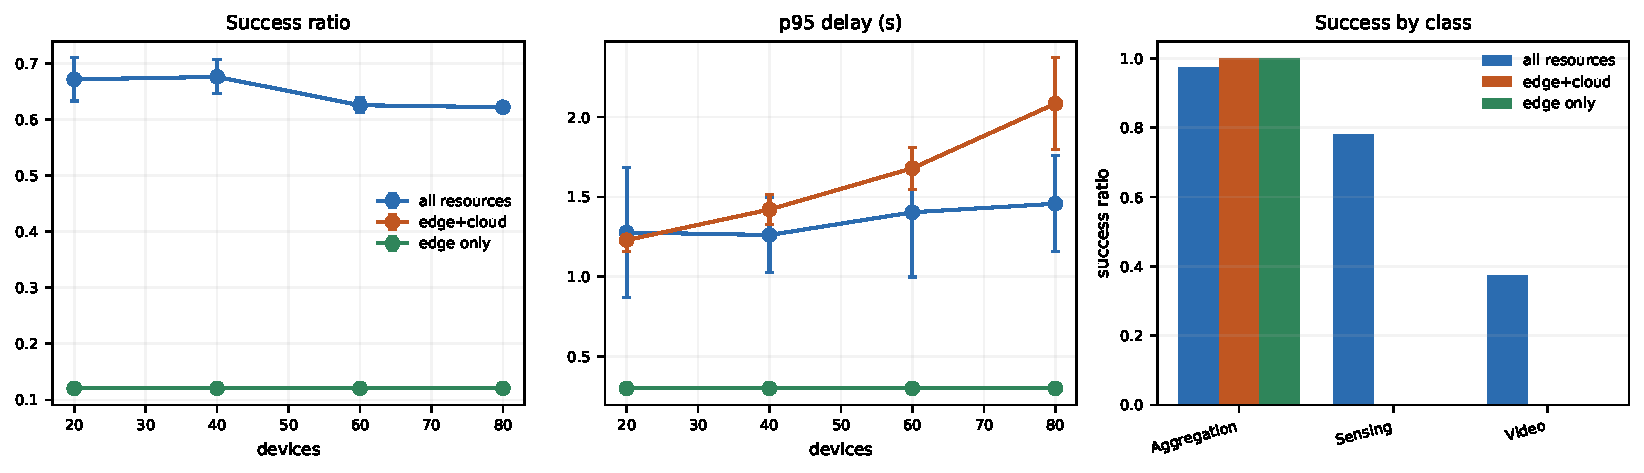
\includegraphics[width=\textwidth]{consolidated/f4.pdf}
\caption{Main performance. (a) success ratio and (b) p95 end-to-end delay against
fleet size, with 95\% confidence bands over seeds; (c) success by application
class and deployment configuration. Patterns: \textsc{all resources},
\textsc{edge+cloud}, \textsc{edge only}.}
\label{fig:new-f4}
\end{figure*}

Table~\ref{tab:effect-guide} disambiguates the closely related values quoted in
this paper. They are different populations, not inconsistent measurements.

\begin{table}[t]
\centering
\footnotesize
\caption{Reading guide to the architecture-effect values quoted in this paper.}
\label{tab:effect-guide}
\begin{tabular}{@{}llc@{}}
\toprule
Value & Subset / statistic & Recomputed\\
\midrule
0.539 & canonical (40 devices, \textsc{trade\_off}, 1~s) & 0.5397\\
0.540 & same effect, paired-seed section & 0.5397\\
0.528 & class share, \emph{not} an effect & 0.528\\
0.648 & \textsc{all} pooled over scale grid & 0.6485\\
\bottomrule
\end{tabular}
\end{table}

\subsection{Application-class decomposition}
Figure~\ref{fig:new-f4}(c) reduces the pooled effect to class feasibility. The
sensing class ($0.528$ of requests) succeeds on $0.779$ under \textsc{all} and
$0.000$ under the two lower configurations; video ($0.352$) reaches $0.374$ and
$0.000$; aggregation ($0.121$) succeeds on $0.975$ everywhere. Recomposing,
$0.121\times0.975+0.528\times0.779+0.352\times0.374=0.661$, matching the pooled
$0.660$. Table~\ref{tab:p1-budget} shows why: tasks finish in $0.025$~s yet fail
because execution starts $1.01$~s after release on an edge site.

\begin{table*}
\centering
\scriptsize
\caption{Delay budget by class and destination at the default 1 s control interval (ALL architecture, 40 devices, 10 seeds). Lag is execution start minus release.}
\label{tab:p1-budget}
\begin{tabular}{llccccccc}
\toprule
Class & Destination & n & Success & Lag (s) & CPU (s) & Net (s) & Deadline (s) & Started \\
\midrule
Aggregation & cloud & 22.286 & 1.000 & 2.120 & 0.200 & 0.880 & 60 & 0.093 \\
Aggregation & edge DC & 64.700 & 1.000 & 1.279 & 0.250 & 0.057 & 60 & 0.270 \\
Aggregation & mist & 153.800 & 1.000 & 0.209 & 1.069 & 0.010 & 60 & 0.641 \\
Sensing & cloud & 42.200 & 0.000 & 2.120 & 0.020 & 0.505 & 0.200 & 0.040 \\
Sensing & edge DC & 69.700 & 0.000 & 1.010 & 0.025 & 0.022 & 0.200 & 0.066 \\
Sensing & mist & 938.100 & 0.870 & 0.131 & 0.110 & 0.003 & 0.200 & 0.893 \\
Video & cloud & 36.400 & 0.000 & 2.120 & 0.120 & 1.025 & 0.800 & 0.052 \\
Video & edge DC & 123.800 & 0.000 & 1.010 & 0.150 & 0.062 & 0.800 & 0.177 \\
Video & mist & 539.800 & 0.481 & 0.475 & 0.486 & 0.029 & 0.800 & 0.771 \\
\bottomrule
\end{tabular}
\par\vspace{2pt}{\footnotesize\raggedright Lag is release to execution start, averaged only over tasks that actually began: tasks killed before dispatch have no start timestamp and are excluded (the Started column gives the retained share). Every infrastructure placement waits roughly one control tick before execution; mist placements start at release.\par}
\end{table*}


The lag is conditional on execution having started; tasks that never started are
excluded, so it must not be read as the average delay experienced by every
generated task.

\subsection{Temporal resolution, deadlines and workload composition}
Figure~\ref{fig:new-f5} consolidates the three sensitivity sweeps. Panel (a) is
the central result: at $1$~s the architecture effect is $+0.5397$, at $0.2$~s it
is $+0.4149$, and at $50$~ms it is $-0.0041$. Panel (b) shows the same effect
collapsing to $+0.0109$ when every deadline is scaled by $16$ while the tick is
unchanged. Panel (c) shows edge-only success tracking the aggregation share
($0.030$, $0.068$, $0.121$, $0.186$, $0.444$ for mixes m1--m5) while
\textsc{all} stays near $0.7$. The mechanism is the tick, not the workload.

\begin{figure*}[t]
\centering
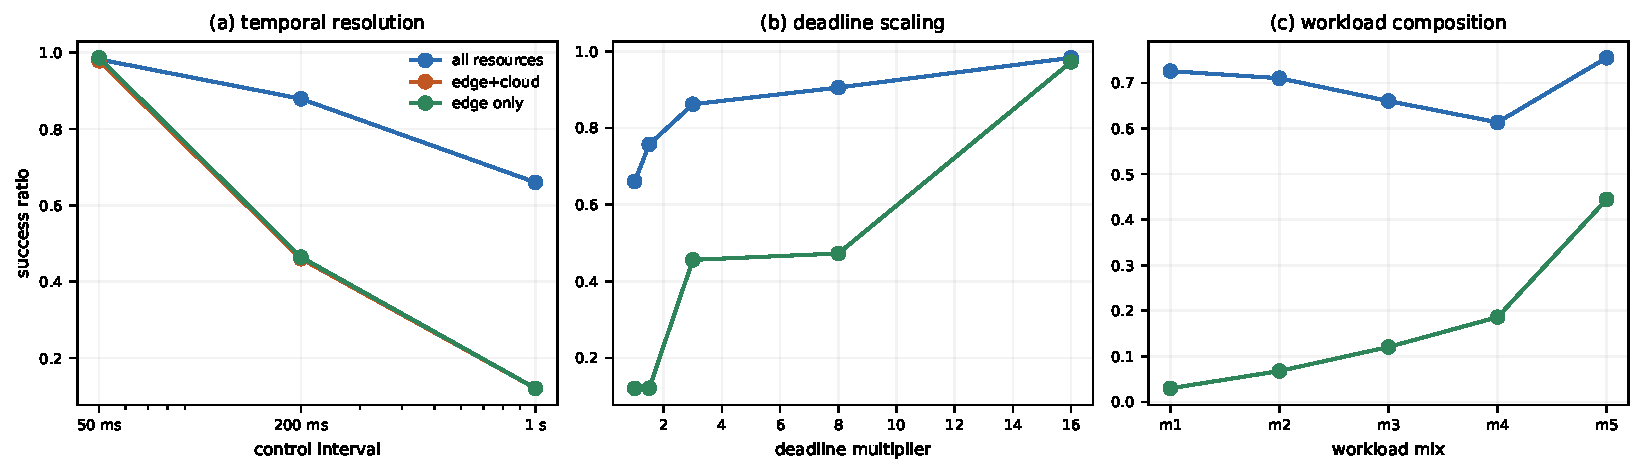
\includegraphics[width=\textwidth]{consolidated/f5.pdf}
\caption{Sensitivity analysis. (a) success against control interval (log axis);
(b) against deadline multiplier; (c) against workload composition. Each curve
is a deployment configuration; 10 seeds per cell, 95\% confidence bands where
the seed variance is resolvable.}
\label{fig:new-f5}
\end{figure*}

\subsection{Latency decomposition and measured calibration}
Figure~\ref{fig:new-f6} separates the components of the delay and replaces the
``$D/10$'' rule of thumb with a measured relation. Release-to-decision and
decision-to-dispatch are zero in this harness; the wait appears entirely between
dispatch and execution start, in whole control intervals. At $1$~s it is
$1.01$~s under earliest-finish, $2.12$~s under least-loaded and $5.07$~s for the
video class under min-min. Deciding itself costs $0.150$--$0.518$~ms, $0.6$--$3.0\%$
of wall clock. Panel (b) plots success against $\rho=L_{\text{decision}}/D$:
stable to $\rho\approx0.5$, collapsing above $\rho>1$. This quantity is
measurable on any engine that timestamps release, decision, dispatch and
execution --- which is why the procedure in Section~\ref{sec:calibration} is the
paper's reusable contribution.

\begin{figure*}[t]
\centering
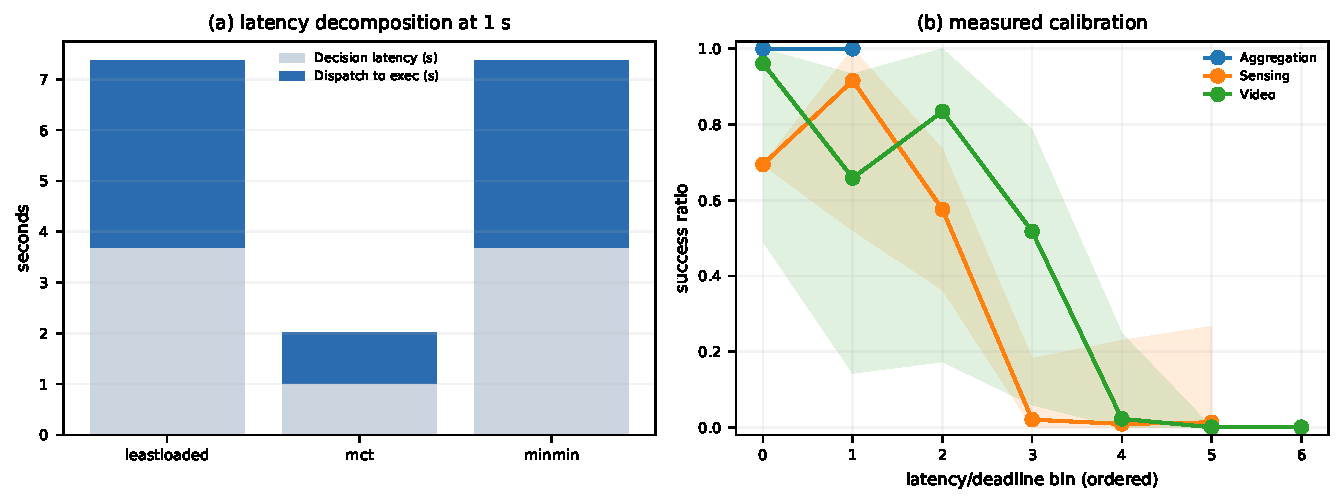
\includegraphics[width=\textwidth]{consolidated/f6.pdf}
\caption{Latency decomposition and calibration. (a) components of the wait for
three representative placement rules at the 1~s tick; (b) success against the
measured latency-to-deadline ratio, with the observed range per bin.}
\label{fig:new-f6}
\end{figure*}

\subsection{Algorithms, infrastructure and placement}
Figure~\ref{fig:new-f7} combines the algorithm and infrastructure evidence.
Panel (a) shows the success heatmap for seven algorithms and three intervals;
rankings invert (Kendall $\tau=0.103$ between $1$~s and $50$~ms, winner changes
from round-robin to earliest-finish). Panel (b) shows the architecture effect
across four infrastructure profiles: at $1$~s it is $+28$ to $+34$ points under
every profile, but at $50$~ms its sign follows the capacity gap ($+65.7$ points
with weak edge and fast cloud, $-3.6$ to $-19.6$ otherwise). Panel (c) shows the
placement distribution that mediates this: the gain is a shift from an
overloaded mist tier to the edge tier.

\begin{figure*}[t]
\centering
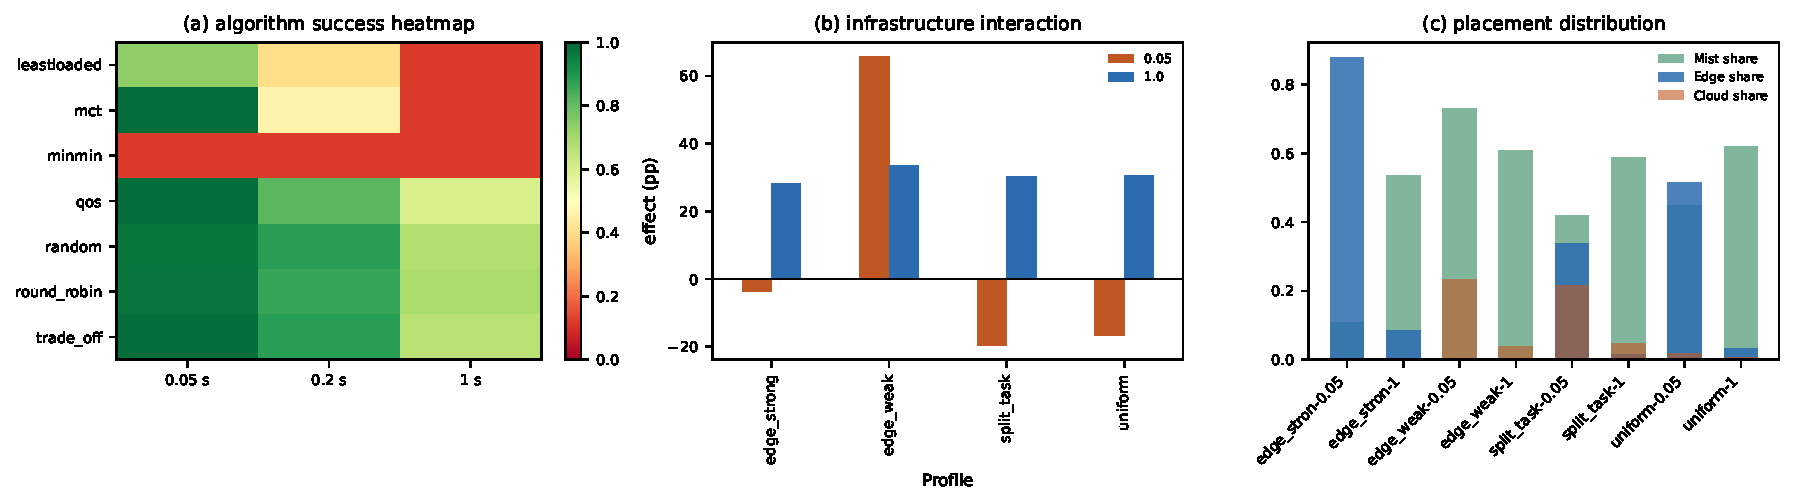
\includegraphics[width=\textwidth]{consolidated/f7.pdf}
\caption{Algorithm and infrastructure effects. (a) algorithm success heatmap at
the full architecture; (b) architecture effect by infrastructure profile and
interval; (c) mist/edge/cloud share of successful tasks under the four profiles.}
\label{fig:new-f7}
\end{figure*}

The three-way ANOVA over the $1{,}680$-run crossed design confirms the
interaction: profile $\times$ interval has partial $\eta^2=0.256$ and the
three-way profile $\times$ architecture $\times$ interval term $\eta^2=0.138$.
The compact model summary is Table~\ref{tab:p1-factor-effects}; the full ANOVA
tables are in the supplement. Note that partial $\eta^2$ is computed from
seed-level aggregates, with runs as the experimental unit; the residual
variance is small because seeds are matched across arms.

\begin{table*}
\centering
\footnotesize
\caption{Factorial analysis of the success ratio over the fully crossed algorithm x architecture x interval design (630 runs, balanced).}
\label{tab:p1-factor-effects}
\begin{tabular}{lcccccc}
\toprule
Term & df & Sum of squares & Mean square & F & p\_value & Partial eta sq \\
\midrule
architecture & 2.000 & 3.382 & 1.691 & 3843.853 & 0.000 & 0.931 \\
policy & 6.000 & 10.512 & 1.752 & 3982.420 & 0.000 & 0.977 \\
update\_interval & 2.000 & 45.088 & 22.544 & 51,242 & 0.000 & 0.994 \\
architecture x update\_interval & 4.000 & 4.276 & 1.069 & 2429.876 & 0.000 & 0.945 \\
policy x architecture & 12 & 7.802 & 0.650 & 1477.837 & 0.000 & 0.969 \\
policy x update\_interval & 12 & 2.801 & 0.233 & 530.481 & 0.000 & 0.918 \\
policy x architecture x update\_interval & 24 & 2.748 & 0.115 & 260.296 & 0.000 & 0.917 \\
Residual & 567 & 0.249 & 0.000 & -- & -- & -- \\
Total & 629 & 76.860 & -- & -- & -- & -- \\
\bottomrule
\end{tabular}
\par\vspace{2pt}{\footnotesize\raggedright The design is perfectly balanced, so each term's sum of squares is the unique ANOVA sum of squares and does not depend on the order of entry. The significant three-way interaction is the formal statement that algorithm comparisons are not configuration-free.\par}
\end{table*}


\subsection{Failures, energy and network behaviour}
Figure~\ref{fig:new-f8} consolidates the failure and resource evidence. Deadline
violations dominate: dependency, resource and device-death failures are zero in
this workload, which is itself evidence that the independent-task arm does not
exercise service dependencies (Section~\ref{sec:app-model}). The energy panels
show the denominator effect: energy per \emph{successful} task ranks
architectures by their success rate, while energy per \emph{generated} task is
comparable. Network sensitivity shows success invariant to WAN latency and
Wi-Fi bandwidth while p95 delay responds, so the binding constraint is the
orchestration delay rather than transmission.

\begin{figure*}[t]
\centering
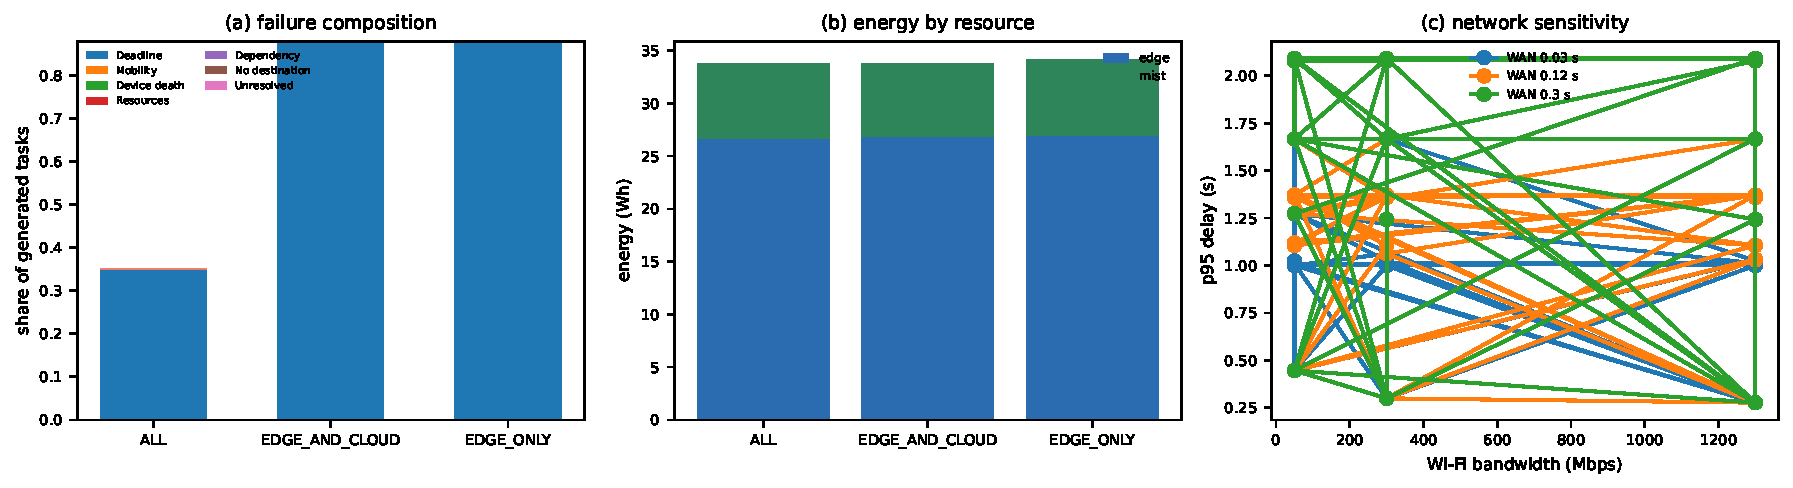
\includegraphics[width=\textwidth]{consolidated/f8.pdf}
\caption{Failure, energy and network behaviour. (a) failure composition by
deployment configuration; (b) energy attributed to edge and mist resources;
(c) p95 delay over the network grid.}
\label{fig:new-f8}
\end{figure*}

\subsection{Workload and mobility robustness}
Figure~\ref{fig:new-f9} keeps the scientifically important distinctions between
the four workload arms. The native trace reaches $0.921$/$0.834$/$0.885$ for the
three configurations; the rate-matched arm reaches $0.948$ (load is not the
explanation, $+2.7$ points), while the deadline-matched arm drops to $0.560$
($-36.1$ points). Mobility affects \textsc{all} ($0.596$--$0.660$ across four
models) but not the lower configurations, because the hosts whose mobility would
matter are not eligible.

\begin{figure*}[t]
\centering
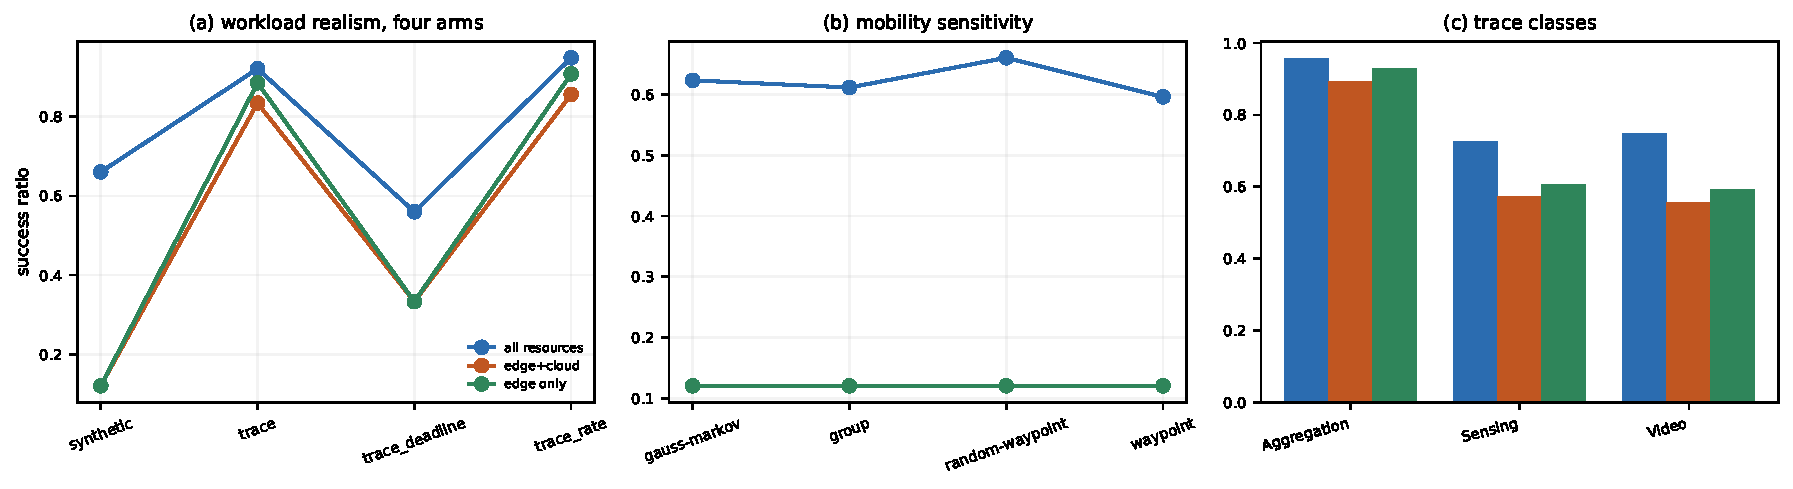
\includegraphics[width=\textwidth]{consolidated/f9.pdf}
\caption{Robustness. (a) success for synthetic, native, rate-matched and
deadline-matched workloads; (b) mobility models; (c) trace success by class.
Rate matching and deadline matching are distinct manipulations and are not
merged.}
\label{fig:new-f9}
\end{figure*}

\subsection{Cross-port audit and cross-simulator validation}
Figure~\ref{fig:new-f10} reports the cross-simulator result on the common trace
and preserves the distinction between executed experiments and unavailable
cells. YAFS reproduces the artefact ($+47.6$ points at $1$~s, $0.0$ at $50$~ms);
EdgeCloudSim, whose placement is a synchronous per-task function with no global
period, serves every class and cannot exhibit it. iFogSim2 is absent: its
adapter is documented as partially implemented and its forwarding defect
recorded at vendored commit \texttt{5f68d394} in
\texttt{crosssim/adapters/ifogsim2/BUG\_REPORT.md}. The independent YAFS
replication (three seeds, a separate experiment) is reported in the supplement
and is not merged with the common-trace result. The Java/Python comparison is a
cross-port audit of one framework, not an independent simulator comparison.

\begin{figure*}[t]
\centering
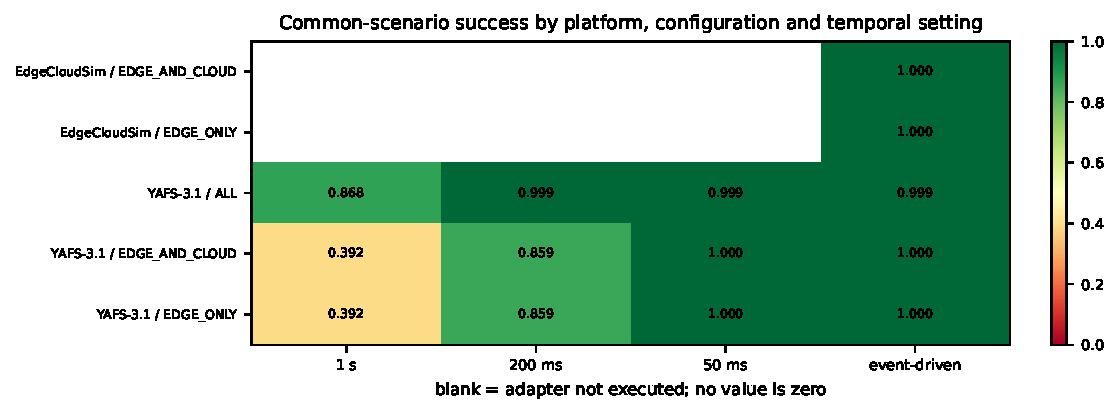
\includegraphics[width=0.9\textwidth]{consolidated/f10.pdf}
\caption{Common-scenario success by platform, deployment configuration and
temporal setting. Blank cells are unavailable experiments, not zeros. The
shared trace was consumed by every executed adapter.}
\label{fig:new-f10}
\end{figure*}

\subsection{Benchmark cost}
Wall-clock runtime grows sub-linearly with fleet size and is reported in
Figure~\ref{fig:runtime}. Decision cost is $0.150$--$0.518$~ms per call, so the
simulated wait is three orders of magnitude larger than the computation that
produces the decision. With four engines now in scope, runtime is also a
comparative metric; we report it for the reference platform only and do not
infer cross-simulator efficiency from incomparable instrumentation.

\begin{figure}[t]
\centering
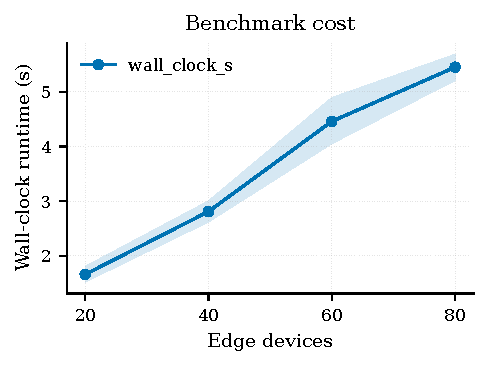
\includegraphics[width=\columnwidth]{f9_runtime.pdf}
\caption{Wall-clock runtime per run against fleet size on the reference platform.}
\label{fig:runtime}
\end{figure}

\paragraph{Supplementary material.}
The complete numerical matrices behind the figures above, the full ANOVA tables,
the seed-level comparisons, and both cross-simulator experiments are in
\texttt{paper/supplementary.tex}. Every value there is generated from the same
artifact as the figures; the main paper retains only the specification tables,
the compact statistical summary and the reading guide needed to interpret the
reported effects.

\section{Discussion}
\label{sec:discussion}

\emph{Why the arithmetic did not catch this.} The per-class table was fully
consistent with a feasibility story: one class succeeds, two do not, and the
pooled ratio is their weighted average. Consistency is not causation, and the
discriminating measurement was the delay budget---a task that meets its compute
deadline and fails anyway. Benchmarks should report that budget by default,
because it is the one table that separates ``cannot'' from ``did not get the
chance''.

\emph{What a calibrated benchmark would have said---and what it would have
missed.} At $50$~ms on a homogeneous fleet the three architectures are within
$0.4$ points, and the honest reading is that architecture does not matter: the
edge tier alone serves $98.7\%$ of requests. That was our earlier conclusion,
and the heterogeneity experiment shows it was too strong. On a fleet whose edge
is weak and whose cloud is fast, the same calibrated benchmark reports $+65.7$
points: the architecture matters a great deal, and the mis-calibrated run
reported only half of it ($+33.6$). The clock is therefore not simply an
optimistic bias that manufactures effects; it is noise on the sign and the size
of an effect that is real in some regimes.

\emph{What the cross-simulator evidence adds.} The common-scenario adapters
answer RQ2 without overstating it. The artefact is not a property of edge
simulators in general: it requires a periodic global placement decision. YAFS,
with the tick injected by our adapter, shows the same collapse as PureEdgeSim;
EdgeCloudSim, which decides at task release, serves every class under the same
trace. iFogSim2's one-shot module placement is likewise incapable of the
artefact by construction, but its adapter has not been executed and it is
therefore not a result in this paper. The generalisation claim is consequently
scoped to engines with a global control period, and the capability matrix makes
the scope auditable.

\emph{What the application model adds.} The dependency-aware arm answers the
reviewer's question about zero dependency failures: the original workload has
no dependencies by construction, so the failure table cannot exercise them.
Service-level DAGs, intermediate transfers and workflow completion are now first
class, with the application graph published independently of the infrastructure
(Figure~\ref{fig:app}). A benchmark that reports microservice orchestration
without such a graph is measuring independent tasks.

\emph{What survives.} The energy denominator effect is independent of the
interval because it is a property of the metric. The conditional mobility effect
is independent because it is about eligibility. The port divergence is
independent because it is about two implementations of the same model. The
algorithmic ranking does not survive a change of either factor, and reporting it
without the configuration is a mistake the factorial model makes visible.

\emph{The design lesson.} A factor study of orchestration needs three things
simultaneously: a temporal resolution below the deadlines, a capacity profile
that leaves the optimiser something to exploit, and a model that includes the
interaction. Any two of the three produce a confident and wrong answer, and our
first two drafts are the demonstration.

% =========================================================================
\section{Threats to Validity}
\label{sec:threats}

\paragraph{Construct validity}
Success counts tasks, not user outcomes, and the classes are proxies. The clock
finding depends on the port invoking the orchestrator on the update tick; a port
that scheduled placements asynchronously would not show the same lag, which is
precisely why the lag should be measured rather than assumed.

\paragraph{Internal validity}
The placement cache is left at its default, so a device's application can be
pinned to its first destination. This is deliberate (it is what a reproducer
would obtain) but it means the destination mix is partly a caching artefact.
The clock comparison holds the cache fixed across intervals, so the causal
inference about the interval is unaffected.

\paragraph{External validity}
The topology is $500\times500$~m with three edge sites and one cloud; there is no
satellite backhaul, no aerial base station and no UAV energy model. The paper is
about multi-tier edge orchestration and its calibration, not about SAGIN, and
the title says so. The replication in Section~\ref{sec:crosssim} covers two independent platforms on the common scenario (YAFS and EdgeCloudSim);
iFogSim2 was built at vendored commit
\texttt{5f68d3947e450d8d2b4af42670be819206be68c9} and source-verified but its
adapter's tuple-to-actuator path failed on that version; the defect is reported
with a reproduction in \texttt{crosssim/adapters/ifogsim2/BUG\_REPORT.md}, and
iFogSim2 is excluded from the experimental comparison rather than assumed to
agree. The
dependency-aware workflow arm is specified and its trace generated, but the
cross-simulator results reported here use the independent-task arm; workflow-level
completion and dependency violations are therefore a specification contribution
at this stage, not a measured result. Absolute success ratios are not expected to
transfer between platforms, and we only claim the effect of the clock.

\paragraph{Conclusion validity}
Ten seeds per cell support the large effects and not differences below about two
percentage points; the network grid uses five seeds, adequate for an invariance
that is exact at the printed precision. The parity audit uses five seeds and one
configuration: it establishes that a divergence exists, not its distribution.

\paragraph{Reproducibility}
The determinism check passes exactly. The simulator version is pinned and
recorded, but floating-point agreement at the last digit depends on the Python
and NumPy versions, which the manifest also records.

% =========================================================================
\section{Conclusion}
\label{sec:concl}

RQ1 is answered by the crossed benchmark: the 1 s control interval manufactured
the $0.539$ architecture effect, which collapses to $-0.004$ at 50 ms, and the
delay-budget evidence identifies the mechanism. RQ4 is answered by the algorithm
grid: rankings invert with the clock (Kendall $\tau=0.103$) and with the
infrastructure profile. RQ3 is answered by the dependency-aware application
model, the four trace arms and the heterogeneity profiles: the architecture
effect changes sign with the capacity gap, and a workload with no dependencies
cannot report dependency failures. RQ2 has a bounded answer: on a shared trace,
YAFS reproduces the artefact while EdgeCloudSim cannot exhibit it because it has
no global control period; iFogSim2 was built and source-verified but its adapter
was not executed, so we make no experimental claim for it. RQ5 is a measured
calibration: report the ratio of decision latency to deadline and compare only
where it is below one half. Deciding costs $0.15$--$0.52$~ms, so the ratio is a
property of the engine, not of the algorithm. The regime map the artefact had
hidden remains the substantive result: on a homogeneous fleet, calibrated, the
architecture does not matter; on a fleet whose edge cannot meet the deadlines it
is worth $65.7$ points, and the uncalibrated run reports half of that.

What remains open is the port. Structural parity fails, the divergence is
localised to mobility and wide-area accounting but not attributed, and closing
it needs a trace replayed identically in both implementations. We report it as a
measured defect rather than a hypothesis, because a benchmark that cannot say
where its two ports disagree cannot claim to be a benchmark of the model rather
than of the port.

\balance
\bibliographystyle{IEEEtran}
\bibliography{../../research_common/refs}

\end{document}
